%% HiPC Student Research Symposium -- 2-page submission (IEEE conference style)
%% Compile with pdflatex (IEEEtran.cls, tikz).
\documentclass[conference]{IEEEtran}
\IEEEoverridecommandlockouts
% The preceding line is only needed to identify funding in the first footnote. If that is unneeded, please comment it out.
%Template version as of 6/27/2024

\usepackage{cite}
\usepackage{amsmath,amssymb,amsfonts}
\usepackage{algorithmic}
\usepackage{graphicx}
\usepackage{textcomp}
\usepackage{xcolor}
\usepackage{booktabs}
\usepackage{tikz}
\usetikzlibrary{arrows.meta,positioning,fit,backgrounds}
\def\BibTeX{{\rm B\kern-.05em{\sc i\kern-.025em b}\kern-.08em
    T\kern-.1667em\lower.7ex\hbox{E}\kern-.125emX}}
\begin{document}

\title{Scaling LLM Serving Simulators with Shared Execution Templates - CHANGE TITLE}

\author{\IEEEauthorblockN{Aryan Bethmangalkar\textsuperscript{*}, Atharva Pandit\textsuperscript{*}, Arnab K. Paul}
\IEEEauthorblockA{\textit{DaSH Lab, Department of CSIS}\\
BITS Pilani K. K. Birla Goa Campus, India\\
\{f20230433, f20230987, arnabp\}@goa.bits-pilani.ac.in}
\and
\IEEEauthorblockN{A, B, C}
\IEEEauthorblockA{\textit{Company Name}\\
City, Country\\
\{name1, name2, name3\}@company.com}
\thanks{\textsuperscript{*}Equal contribution.}
}


\maketitle

\begin{abstract}
LLM serving simulators such as LLMServingSim hand each batch to a network
simulator as one execution trace file per accelerator, so their own cost
grows with the simulated cluster. Swapping the files for in-memory buffers
made the simulator 2.4 times slower, because the cost lies in redundant
work and memory management. The ranks of a batch run nearly identical
graphs, and identical instances keep producing the same batch shapes. We
send each batch as one shared \emph{execution template} plus a small
per-rank overlay and reuse templates across instances; the network
simulator builds every rank's graph on the shared template. At 256
accelerators, simulation time falls by 47\% and file system traffic from
39.8 GB to 4.8 MB, while simulated results stay byte-identical.
\end{abstract}

\begin{IEEEkeywords}
LLM inference, simulation, scalability
\end{IEEEkeywords}

\section{Introduction}

\textbf{Objective.} LLM serving systems such as vLLM~\cite{vllm} group
requests from many users into \emph{batches} and run them on clusters of
hundreds of accelerators. Exploring cluster designs on real hardware at
that scale is too expensive, so researchers use
simulators to predict latency and throughput. The most faithful
simulators pair a \emph{serving model}, which decides which requests run
together, with a \emph{network simulator}, which predicts how long the
resulting computation and communication take
(Section~\ref{sec:design}). Our objective is to scale the simulator to hundreds of accelerators on a single server by eliminating redundant per-rank execution-trace traffic between its serving model and network simulator.

\textbf{Limitations of the state of the art.} The bottleneck lies in the
trace-driven interface that high-fidelity simulators share. The widely
used network simulator ASTRA-sim~\cite{astrasim2} reads one Chakra
\emph{execution trace}~\cite{chakra} per simulated accelerator: a file
listing the operations that accelerator performs and the order they must
follow. Any serving simulator built on it must write traces at every
scheduling step.

LLMServingSim~\cite{llmservingsim}, built on ASTRA-sim, writes one trace
per accelerator per batch, 39.8\,GB of transient files for 750 requests
at 256 accelerators. Passing these traces through in-memory buffers
instead of files made it 2.4$\times$ slower in our measurements, because
the per-rank duplication and memory management that dominate the cost
remain. Simulators that avoid traces altogether give up the network
model: Vidur~\cite{vidur} and roofline-based simulators estimate
communication from measured profiles or peak-bandwidth formulas, which
cannot capture how topology or competing traffic slows a transfer.


\textbf{Key insights and contributions.} (i)~\emph{Rank redundancy:} the
ranks of a batch run the same graph except for a few communication-peer
fields, so a batch can be represented once as a shared structure plus a
small per-rank overlay. (ii)~\emph{Instance redundancy:} identical
instances keep producing the same batch shapes, so a template cache keyed
on batch shape rather than accelerator numbers lets one instance reuse
another's work. (iii)~\emph{Memory management:} the network simulator's
main overhead over the baseline (LLMServingSim) is copying and allocating graph nodes,
which sharing structures across ranks and a better-suited allocation
policy largely remove. We contribute an execution-template design built
on these observations, validated to produce byte-identical results, and
an evaluation from 16 to 256 accelerators.


\textbf{Limitations.} The benefit tracks the number of identical
instances, so small deployments gain least (19.1\% at 16 accelerators). The
serving model and the network simulator still take turns instead of
overlapping, we do not yet support data-parallel groups, and all
measurements come from a single host.

\section{Design}
\label{sec:design}

\textbf{Background.} The simulator replays a stream of user requests against a model of a cluster of
accelerators. The cluster
is divided into \emph{instances}, identical copies of the LLM that each
serve a share of the requests. A model too large for one accelerator is split
with \emph{tensor parallelism}: every layer is divided among the accelerators of
an instance, each called a \emph{rank} (TP4 means four ranks per
instance), and the ranks combine partial results through a collective communication
operation, the \emph{all-reduce}. At each simulation step, the serving
model forms a batch and describes it as one
\emph{dependency graph} per rank, whose nodes are compute or
communication operations and whose edges say which must finish first.
The network simulator executes these graphs event by event and reports
the elapsed simulated time. In LLMServingSim, each graph is written to
disk as a trace file, so every step produces one file per accelerator. Our design (Fig.~\ref{fig:design}) replaces these files with four components.

\textbf{Structure/overlay representation.} Within a batch, every rank's
graph has the same operations in the same order. The graphs differ only
in a few fields, chiefly which accelerators each communication operation talks
to. We split each batch into one \emph{structure}, common to all ranks,
and a small per-rank \emph{overlay} holding the fields that differ.
Together they form an \emph{execution template}. The structure is
immutable and named by a hash of its contents, so when the network
simulator already holds a structure, the serving model sends only its
name.

\textbf{Placement-independent template cache.} In a homogeneous setup, instances of the same
model often receive batches of the same shape (the same mix of request
lengths). These yield identical templates, except that one instance's
accelerators might be numbered 12--15 and another's 28--31. The serving model
looks templates up with a key that leaves out accelerator numbers, and
on a hit it only renumbers the overlays.
More instances produce more repeated
shapes, so reuse grows with deployment size.

\textbf{Shared graph construction.} The network simulator keeps recently
used structures in a fixed-size cache and frees one only when no rank still
uses it. It builds each rank's graph on top of the shared structure
rather than on a private copy, so per-rank memory only covers what differs.

\textbf{Allocation policy.} For each batch, the network simulator
makes a few large allocations and millions of small ones for graph
nodes. By default, glibc keeps freed small blocks in a fast-reuse cache
and merges them into its main free lists only when a large block is
requested, so each large allocation pays for every small block freed
since the previous one. Profiling showed this was the network
simulator's main extra cost over the baseline. With
\texttt{mallopt(M\_MXFAST,\,0)}, small blocks merge as they are freed.


\begin{figure}[t]
\centering
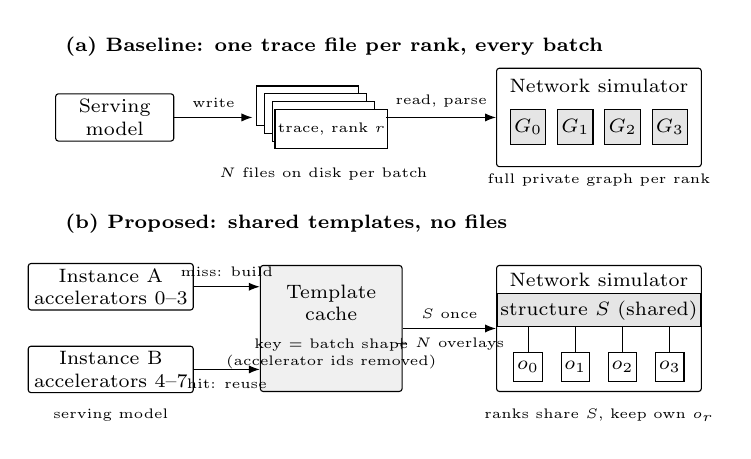
\begin{tikzpicture}[
  font=\scriptsize,
  box/.style={draw,rounded corners=1pt,align=center,inner sep=2pt},
  file/.style={draw,fill=white,minimum width=1.3cm,minimum height=0.5cm,inner sep=1pt},
  graph/.style={draw,fill=black!10,minimum size=0.45cm,inner sep=0pt},
  ovl/.style={draw,fill=white,minimum size=0.36cm,inner sep=0pt},
  ar/.style={-{Latex[length=1.4mm]}},
  lbl/.style={font=\tiny}]

%% (a) baseline
\node[anchor=west,font=\scriptsize\bfseries] at (0,0.9) {(a) Baseline: one trace file per rank, every batch};
\node[box,minimum width=1.5cm,minimum height=0.6cm] (sm1) at (0.75,0) {Serving\\model};
\foreach \i in {0,1,2} \node[file] at (3.2+0.1*\i,0.15-0.1*\i) {};
\node[file,font=\tiny] (tr) at (3.5,-0.15) {trace, rank $r$};
\node[lbl] at (3.4,-0.72) {$N$ files on disk per batch};
\node[box,minimum width=2.6cm,minimum height=1.25cm] (ns1) at (6.9,0) {};
\node at (6.9,0.4) {Network simulator};
\foreach \i in {0,1,2,3} \node[graph] at (6.0+0.6*\i,-0.12) {$G_{\i}$};
\node[lbl] at (6.9,-0.8) {full private graph per rank};
\draw[ar] (sm1.east) -- node[above,lbl]{write} (2.5,0);
\draw[ar] (4.2,0) -- node[above,lbl]{read, parse} (ns1.west);

%% (b) proposed
\node[anchor=west,font=\scriptsize\bfseries] at (0,-1.35) {(b) Proposed: shared templates, no files};
\node[box,minimum width=1.4cm] (ia) at (0.7,-2.15) {Instance A\\accelerators 0--3};
\node[box,minimum width=1.4cm] (ib) at (0.7,-3.2) {Instance B\\accelerators 4--7};
\node[lbl] at (0.7,-3.78) {serving model};
\node[box,fill=black!6,minimum width=1.8cm,minimum height=1.6cm] (tc) at (3.5,-2.68) {};
\node[align=center] at (3.5,-2.35) {Template\\cache};
\node[lbl,align=center] at (3.5,-3.0) {key = batch shape\\(accelerator ids removed)};
\draw[ar] (ia.east) -- node[above,lbl]{miss: build} (tc.west |- ia.east);
\draw[ar] (ib.east) -- node[below,lbl]{hit: reuse} (tc.west |- ib.east);
\node[box,minimum width=2.6cm,minimum height=1.6cm] (ns2) at (6.9,-2.68) {};
\node at (6.9,-2.06) {Network simulator};
\node[draw,fill=black!10,minimum width=2.3cm,minimum height=0.42cm,inner sep=1pt] (S) at (6.9,-2.45) {structure $S$ (shared)};
\foreach \i in {0,1,2,3} {
  \node[ovl] (o\i) at (6.0+0.6*\i,-3.17) {$o_{\i}$};
  \draw (o\i.north) -- (o\i.north |- S.south);
}
\node[lbl] at (6.9,-3.78) {ranks share $S$, keep own $o_r$};
\draw[ar] (tc.east) -- node[above,lbl]{$S$ once} node[below,lbl]{+ $N$ overlays} (ns2.west);
\end{tikzpicture}
\caption{(a) The baseline writes a full trace file for every rank of every
batch, and the network simulator builds a private graph $G_r$ from each.
(b) Our design sends one shared structure $S$ plus a small overlay $o_r$
per rank holding the fields that differ, such as which accelerators to
communicate with. Instance B reuses a template built for instance A
after renumbering.}
\label{fig:design}
\end{figure}

\section{Evaluation}

\textbf{Testbed and methodology.} All runs use one Linux server and the same 750-request ShareGPT trace at 10
requests/s. We scale a cluster of Llama-3.1-70B instances, each on
four accelerators (TP4), from 4 to 64 instances (16 to 256 simulated accelerators). The
baseline is the same frozen LLMServingSim build with its original
trace-file interface.

\textbf{Results.} Wall-clock time falls by 19.1\% at 16 accelerators and by
47.2\% at 256 (Table~\ref{tab:results}). The saving tracks the
template cache, whose hit rate rises from 58\% to 98\% over that range; there, 99\% of hits reuse a batch first built by another instance.
Most of the gain is in the serving model, whose CPU time falls
9.4$\times$ at 256 accelerators. The network simulator costs 5--6\% more than
the baseline at 16 and 72 accelerators and 22\% less at 256. Data written
to disk drops by three to four orders of magnitude, from 2.91\,GB to
2.4\,MB at 16 accelerators and from 39.8\,GB to 4.8\,MB at 256, and open
descriptors stay at 21 regardless of accelerator count. Peak memory is
4--13\% below the baseline at every scale.


\textbf{Exactness.} Our design changes how a graph reaches the network
simulator but not the graph itself. Every pair of runs in
Table~\ref{tab:results} produced byte-identical per-request results and
the same simulated clock.

\begin{table}[t]
\caption{ShareGPT-750, idle host, identical build. B: baseline;
P: proposed. Serving/Network: CPU time of each component. Written and
FDs: simulator-induced file system traffic and steady-state open
descriptors. Mem: peak resident memory of the simulator's processes.}
\label{tab:results}
\centering
\footnotesize\setlength{\tabcolsep}{3.2pt}
\begin{tabular}{@{}lrrrrrrr@{}}
\toprule
Accelerators & & Wall & Serving & Network & Written & Peak Mem & FDs \\
\midrule
16 (4$\times$TP4)   & B & 4:14 & 129\,s & 121\,s & 2.91\,GB & 228\,MiB & 37 \\
                    & P & \textbf{3:25} & 76\,s & 128\,s & 2.4\,MB & 219\,MiB & 21 \\
72 (18$\times$TP4)  & B & 21:04 & 587\,s & 659\,s & 12.6\,GB & 332\,MiB & 93 \\
                    & P & \textbf{13:15} & 94\,s & 692\,s & 3.1\,MB & 300\,MiB & 21 \\
128 (32$\times$TP4) & B & 41:36 & 1037\,s & 1431\,s & 21.9\,GB & 430\,MiB & 149 \\
                    & P & \textbf{23:24} & 106\,s & 1285\,s & 3.6\,MB & 382\,MiB & 21 \\
256 (64$\times$TP4) & B & 1:20:14 & 1833\,s & 3019\,s & 39.8\,GB & 642\,MiB & 277 \\
                    & P & \textbf{42:22} & 196\,s & 2349\,s & 4.8\,MB & 560\,MiB & 21 \\
\bottomrule
\end{tabular}
\end{table}


\section{Conclusion and Future Work}

Per-rank trace overhead in LLM serving simulators comes mainly from redundant graph construction and allocation, not I/O. Sharing execution templates across ranks and instances removes most of it, cutting wall-clock time by up to 47\% at 256 accelerators with byte-identical results. The largest remaining opportunity is to overlap template preparation with network simulation. We also plan to  validate the design on larger workloads with bigger models.

\begin{thebibliography}{9}
\bibitem{llmservingsim}
J.~Cho \emph{et al.}, ``LLMServingSim: A HW/SW co-simulation
infrastructure for LLM inference serving at scale,'' in \emph{IEEE Int.
Symp. Workload Characterization (IISWC)}, 2024.

\bibitem{astrasim2}
W.~Won \emph{et al.}, ``ASTRA-sim2.0: Modeling hierarchical networks and
disaggregated systems for large-model training at scale,'' in \emph{IEEE
Int. Symp. Performance Analysis of Systems and Software (ISPASS)}, 2023.

\bibitem{chakra}
S.~Sridharan \emph{et al.}, ``Chakra: Advancing performance benchmarking
and co-design using standardized execution traces,'' arXiv:2305.14516,
2023.

\bibitem{vllm}
W.~Kwon \emph{et al.}, ``Efficient memory management for large language
model serving with PagedAttention,'' in \emph{ACM Symp. Operating Systems
Principles (SOSP)}, 2023.

\bibitem{vidur}
A.~Agrawal \emph{et al.}, ``Vidur: A large-scale simulation framework for
LLM inference,'' in \emph{Proc. Machine Learning and Systems (MLSys)},
2024.
\end{thebibliography}

\end{document}
